\subsubsection{Uso por aficionado de los museos}

{\textbf {Resumen:}}
Un cliente habitual de los museos ve un folleto en la mesa principal de la entrada del museo, ve que hay una nueva App que permite ver el museo en su casa y que es interactivo, cuando vuelve a su casa, la descarga, imprime el código y empieza a descubrir cada una de las piezas del museo, fascinado con la aplicacion, comparte en redes sociales cada una de las piezas y el logro que obtuvo por completar el descubrimiento completo de las piezas de los museos regionales.

{\textbf {Actores:}}
Aficionado.

{\textbf {Propósito:}}
Evidenciar la conexión directa entre personas que frecuentas museos y la accesibilidad a la aplicación por parte de folletos dentro de los museos.

{\textbf {Referencias cruzadas:}}
R1.1, R1.2, R1.3, R1.4, R2.2, R2.3, R4.1, R4.2, R4.3, R4.4

\paragraph{Caso de Uso Esencial}

\begin{longtable}{|p{5cm}|p{8cm}|}
\hline 
Acción actores & Respuesta del sistema \\ 
\hline 
XXXX & XXXX \\ 
\hline 
\end{longtable}

\paragraph{Diagrama de Caso de Uso}

\begin{figure}[H]
\centerline{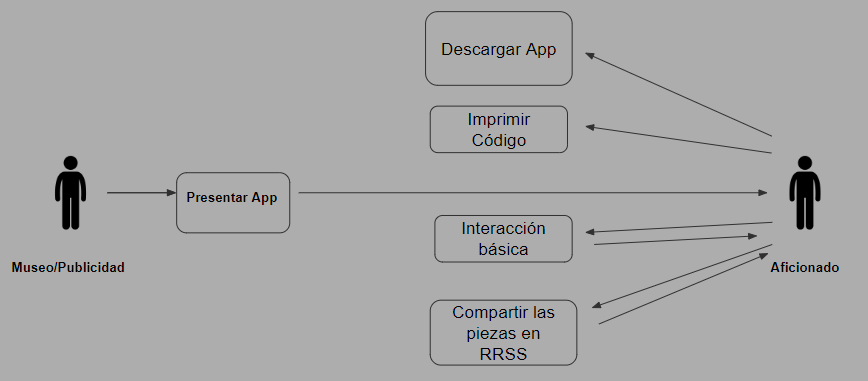
\includegraphics[width=15cm]{imgs/CasoUso_6.PNG}}
\caption{Caso-1}
\label{fig}
\end{figure}

\paragraph{Modelo Conceptual}

\begin{figure}[H]
\centerline{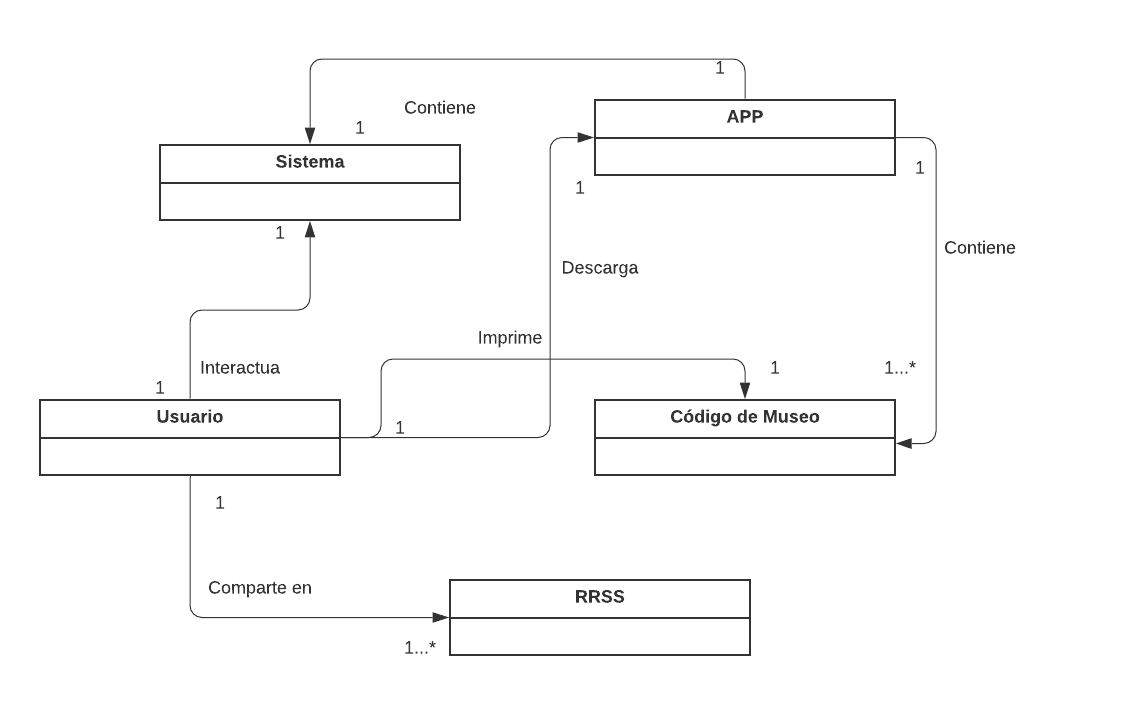
\includegraphics[width=15cm]{imgs/ModeloConceptualCaso_6_3.png}}
\caption{Caso-1}
\label{fig}
\end{figure}

\paragraph{Diagrama de Secuencia o Colaboración}

\begin{figure}[H]
\centerline{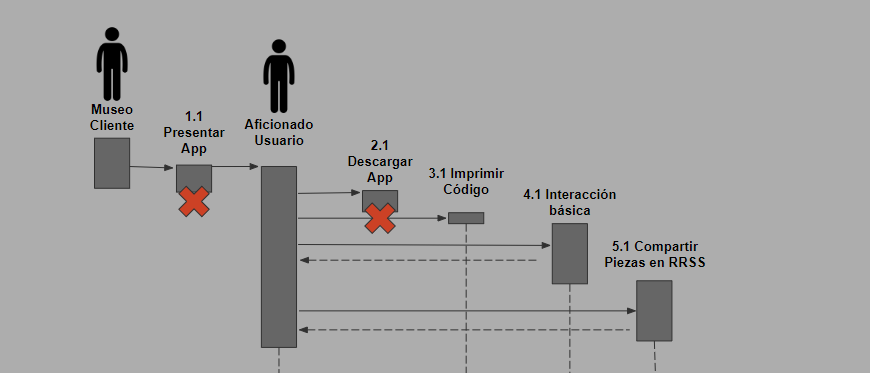
\includegraphics[width=15cm]{imgs/CasoUso_6_2.PNG}}
\caption{Caso-1}
\label{fig}
\end{figure}

\paragraph{Priorización}
{\textbf {Tipo:}}
Principal.